%!TEX root = ../thesis.tex
%*******************************************************************************
%*********************************** First Chapter *****************************
%*******************************************************************************

\chapter{Introduction}  %Title of the First Chapter

\ifpdf
    \graphicspath{{Chapter1/Figs/Raster/}{Chapter1/Figs/PDF/}{Chapter1/Figs/}}
\else
    \graphicspath{{Chapter1/Figs/Vector/}{Chapter1/Figs/}}
\fi


%********************************** %First Section  **************************************
\section{Motivation and challenge \texorpdfstring{}{}} %Section - 1.1 

\noindent Combustion has been integral to human development, evolving from early domestic applications such as heating and cooking, through industrial processes including ore smelting, glass production, and ceramic manufacturing, to modern technologies such as steam engines, transportation systems, and power generation~\citep{Lackner}. The science of combustion itself has a long and well‑established history~\citep{Bilger,Lackner,Allen,Deane,Richardson,Stavrianos}. Today, the combustion of fossil fuels remains the predominant source of global energy and is expected to retain that role for the foreseeable future owing to the sustained availability of resources such as coal.  The BP statistical review of world energy~\citep{BP} reports that fossil fuels accounted for approximately 82\% of primary energy consumption as shown in Figure~\ref{fig:share}. Although renewable energy supply increased by over 8 EJ compared with the previous year, overall fossil‑fuel consumption was not reduced; primary energy demand rose by 5.8\% in 2021 and exceeded 2019 levels by 1.3\%, indicating that fossil fuels are likely to continue to dominate the global energy supply. It is well known that combustion not only generates heat that can be converted into power but also produces pollutants such as nitrogen oxides, soot, and unburnt hydrocarbons~\citep {Peters_2000,lieuwen}. Consequently, the combustion of fossil fuels contributes to environmental degradation and atmospheric pollution through greenhouse gas emissions and toxic species. Increasingly stringent legislations are therefore compelling hard-to-abate sectors, such as aviation, power, and the automotive industry, to reduce pollutant emissions to protect the environment. One approach adopted by these industries is the replacement of conventional hydrocarbon fuels with low or zero carbon alternatives such as hydrogen. 

\begin{figure}[htbp!] 
\centering    
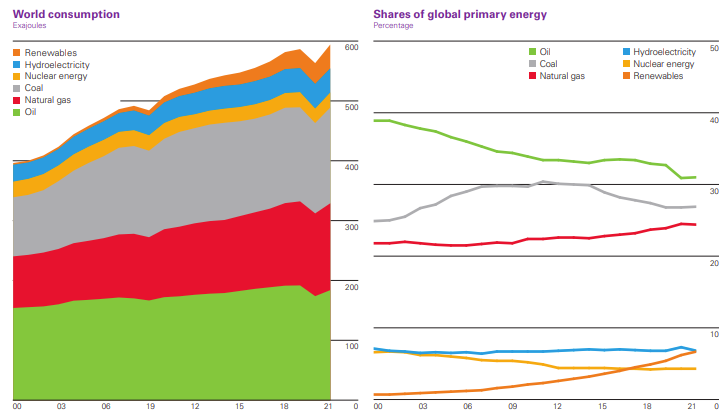
\includegraphics[width=0.5\textwidth]{share1.png}
\caption[share]{Global primary energy consumption by source (EJ and \%)~\citep{BP}}
\label{fig:share}
\end{figure}

Hydrogen combustion systems are gaining increasing attention as a pathway to meet decarbonisation targets and comply with emerging climate policies. However, hydrogen flames present significant challenges for flame stabilisation, as they are characterised by higher burning velocities, thinner reaction zones, and a greater propensity to propagate close to injector lips while often operating in a diffusion mode~\citep{Chaplet}. In addition, hydrogen exhibits a high propensity for spontaneous ignition compared with conventional fuels, further complicating its safe handling and application~\citep{Astbury}. Over the past four decades, the progressive refinement of combustion technologies has been a principal factor in lowering atmospheric pollution in industrialised nations~\citep{Sawyer}. In fact, since the mid-1970, combustion science has advanced substantially in response to demands for energy security and environmental protection, driven by progress in mathematical analysis, computational modelling and experimental techniques~\citep {Law_2006}. However, the use of computational approaches is not without its own challenges, as engineers continue to develop methods to address the complexity of reacting flows and turbulence in practical combustion systems, a complexity that requires a detailed interdisciplinary understanding of thermodynamics, chemical kinetics, fluid mechanics, and transport phenomena~\citep{Law_2006}.

The continued development of computational fluid dynamics (CFD) has significantly enhanced the role of numerical simulation in modern combustion research for both academic and industrial applications~\citep{poinsot}. Numerical simulation enables detailed three dimensional and time dependent analysis of flame structures with accurate chemical and transport models, supporting the understanding and modelling of combustion phenomena~\citep{Mizobuchi2005}. It also provides insight into turbulence chemistry interactions by overcoming limitations associated with experimental measurement techniques~\citep{Gong}, and has therefore been widely employed alongside experimental investigations to study flame stabilisation in turbulent lifted hydrogen jet flames~\citep{Brockhinke,Mizobuchi2005, Mizobuchi2002,Yoo2009,TCheng1992,Schumann2025}. These investigations are typically conducted under lean operating conditions, to improve efficiency, reduce flame temperatures and thereby reduce pollutant emissions \citep {Driscoll2011,Massey2019}, although such conditions also increase susceptibility to ignition failure and flame instability~\citep{Gicquel2012}. 

\begin{figure}[htbp!] 
\centering    
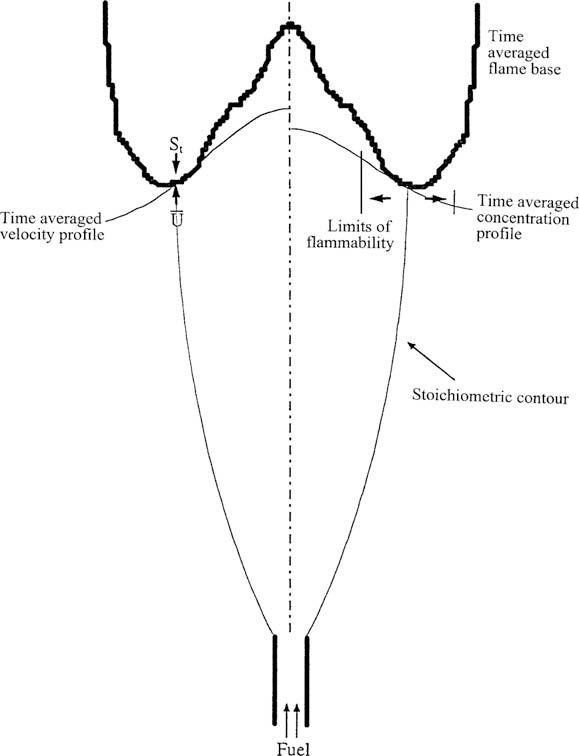
\includegraphics[width=0.3\textwidth]{share2.jpg}
\caption[share1]{Schematic diagram of the lifted flame~\citep{Lawn2009}}
\label{fig:share1}
\end{figure}

Combustion frequently involves the interaction of a fuel and an oxidiser, and the way these reactants are mixed determines the type of flame formed, strongly influencing the combustion behaviour~\citep {Law_2006}. The mode of mixing between fuel and oxidiser determines the type of flame formed and consists of premixed combustion in which reactants are initially mixed, non-premixed mode in which mixing occurs through molecular diffusion, and partially premixed combustion which arises in practical turbulent systems due to incomplete mixing prior to ignition, making the understanding of flame stabilisation mechanisms essential~\citep{Peters_2000,Law_2006,Syred2006}. 

Flames in large industrial boilers and gas turbines are commonly stabilised using non premixed jet configurations, with swirling flows employed to extend the range of flame stability in combustion systems; however, as this research does not consider swirl stabilised flows, the reader is referred to the relevant literature for further discussion~\citep{Massey2022,Feikema1990}. The turbulent lifted hydrogen jet flame arises under conditions of partially premixed combustion and is characterised by a separation between the flame stabilisation root and the burner nozzle, defined as the lift off height H, as shown in Figure~\ref{fig:share1}. This configuration involves fuel injected into quiescent air, forming inhomogeneous mixtures where the flame remains attached at low jet velocities but stabilises downstream at higher velocities due to turbulence and local extinction~\citep{Peters_2000}, and is commonly preferred in practical systems to protect the burner nozzle~\citep{Mansour2003}. In a turbulent lifted jet flame, uneven mixing occurs upstream of the flame root, leading to different combustion behaviours at various locations. Hence, combustion is said to be multi-modal~\citep{Schumann2025,Mizobuchi2005,Mizobuchi2002}. 







%********************************** %Second Section  *************************************
\section{Approach and objectives} %Section - 1.2


It is a long established fact that a reader will be distracted by the readable content of a page when looking at its layout. The point of using Lorem Ipsum is that it has a more-or-less normal distribution of letters, as opposed to using `Content here, content here', making it look like readable English. Many desktop publishing packages and web page editors now use Lorem Ipsum as their default model text, and a search for `lorem ipsum' will uncover many web sites still in their infancy. Various versions have evolved over the years, sometimes by accident, sometimes on purpose (injected humour and the like).

%********************************** % Third Section  *************************************
\section{Thesis structure}  %Section - 1.3 
\label{section1.3}

Contrary to popular belief, Lorem Ipsum is not simply random text. It has roots in a piece of classical Latin literature from 45 BC, making it over 2000 years old. Richard McClintock, a Latin professor at Hampden-Sydney College in Virginia, looked up one of the more obscure Latin words, consectetur, from a Lorem Ipsum passage, and going through the cites of the word in classical literature, discovered the undoubtable source. Lorem Ipsum comes from sections 1.10.32 and 1.10.33 of "de Finibus Bonorum et Malorum" (The Extremes of Good and Evil) by Cicero, written in 45 BC. This book is a treatise on the theory of ethics, very popular during the Renaissance. The first line of Lorem Ipsum, "Lorem ipsum dolor sit amet..", comes from a line in section 1.10.32.

The standard chunk of Lorem Ipsum used since the 1500s is reproduced below for those interested. Sections 1.10.32 and 1.10.33 from ``de Finibus Bonorum et Malorum" by Cicero are also reproduced in their exact original form, accompanied by English versions from the 1914 translation by H. Rackham

``Lorem ipsum dolor sit amet, consectetur adipisicing elit, sed do eiusmod tempor incididunt ut labore et dolore magna aliqua. Ut enim ad minim veniam, quis nostrud exercitation ullamco laboris nisi ut aliquip ex ea commodo consequat. Duis aute irure dolor in reprehenderit in voluptate velit esse cillum dolore eu fugiat nulla pariatur. Excepteur sint occaecat cupidatat non proident, sunt in culpa qui officia deserunt mollit anim id est laborum."

Section 1.10.32 of ``de Finibus Bonorum et Malorum", written by Cicero in 45 BC: ``Sed ut perspiciatis unde omnis iste natus error sit voluptatem accusantium doloremque laudantium, totam rem aperiam, eaque ipsa quae ab illo inventore veritatis et quasi architecto beatae vitae dicta sunt explicabo. Nemo enim ipsam voluptatem quia voluptas sit aspernatur aut odit aut fugit, sed quia consequuntur magni dolores eos qui ratione voluptatem sequi nesciunt. Neque porro quisquam est, qui dolorem ipsum quia dolor sit amet, consectetur, adipisci velit, sed quia non numquam eius modi tempora incidunt ut labore et dolore magnam aliquam quaerat voluptatem. Ut enim ad minima veniam, quis nostrum exercitationem ullam corporis suscipit laboriosam, nisi ut aliquid ex ea commodi consequatur? Quis autem vel eum iure reprehenderit qui in ea voluptate velit esse quam nihil molestiae consequatur, vel illum qui dolorem eum fugiat quo voluptas nulla pariatur?"

1914 translation by H. Rackham: ``But I must explain to you how all this mistaken idea of denouncing pleasure and praising pain was born and I will give you a complete account of the system, and expound the actual teachings of the great explorer of the truth, the master-builder of human happiness. No one rejects, dislikes, or avoids pleasure itself, because it is pleasure, but because those who do not know how to pursue pleasure rationally encounter consequences that are extremely painful. Nor again is there anyone who loves or pursues or desires to obtain pain of itself, because it is pain, but because occasionally circumstances occur in which toil and pain can procure him some great pleasure. To take a trivial example, which of us ever undertakes laborious physical exercise, except to obtain some advantage from it? But who has any right to find fault with a man who chooses to enjoy a pleasure that has no annoying consequences, or one who avoids a pain that produces no resultant pleasure?"

Section 1.10.33 of ``de Finibus Bonorum et Malorum", written by Cicero in 45 BC: ``At vero eos et accusamus et iusto odio dignissimos ducimus qui blanditiis praesentium voluptatum deleniti atque corrupti quos dolores et quas molestias excepturi sint occaecati cupiditate non provident, similique sunt in culpa qui officia deserunt mollitia animi, id est laborum et dolorum fuga. Et harum quidem rerum facilis est et expedita distinctio. Nam libero tempore, cum soluta nobis est eligendi optio cumque nihil impedit quo minus id quod maxime placeat facere possimus, omnis voluptas assumenda est, omnis dolor repellendus. Temporibus autem quibusdam et aut officiis debitis aut rerum necessitatibus saepe eveniet ut et voluptates repudiandae sint et molestiae non recusandae. Itaque earum rerum hic tenetur a sapiente delectus, ut aut reiciendis voluptatibus maiores alias consequatur aut perferendis doloribus asperiores repellat."

1914 translation by H. Rackham: ``On the other hand, we denounce with righteous indignation and dislike men who are so beguiled and demoralized by the charms of pleasure of the moment, so blinded by desire, that they cannot foresee the pain and trouble that are bound to ensue; and equal blame belongs to those who fail in their duty through weakness of will, which is the same as saying through shrinking from toil and pain. These cases are perfectly simple and easy to distinguish. In a free hour, when our power of choice is untrammelled and when nothing prevents our being able to do what we like best, every pleasure is to be welcomed and every pain avoided. But in certain circumstances and owing to the claims of duty or the obligations of business it will frequently occur that pleasures have to be repudiated and annoyances accepted. The wise man therefore always holds in these matters to this principle of selection: he rejects pleasures to secure other greater pleasures, or else he endures pains to avoid worse pains."

\nomenclature[z-DEM]{DEM}{Discrete Element Method}
\nomenclature[z-FEM]{FEM}{Finite Element Method}
\nomenclature[z-PFEM]{PFEM}{Particle Finite Element Method}
\nomenclature[z-FVM]{FVM}{Finite Volume Method}
\nomenclature[z-BEM]{BEM}{Boundary Element Method}
\nomenclature[z-MPM]{MPM}{Material Point Method}
\nomenclature[z-LBM]{LBM}{Lattice Boltzmann Method}
\nomenclature[z-MRT]{MRT}{Multi-Relaxation 
Time}
\nomenclature[z-RVE]{RVE}{Representative Elemental Volume}
\nomenclature[z-GPU]{GPU}{Graphics Processing Unit}
\nomenclature[z-SH]{SH}{Savage Hutter}
\nomenclature[z-CFD]{CFD}{Computational Fluid Dynamics}
\nomenclature[z-LES]{LES}{Large Eddy Simulation}
\nomenclature[z-FLOP]{FLOP}{Floating Point Operations}
\nomenclature[z-ALU]{ALU}{Arithmetic Logic Unit}
\nomenclature[z-FPU]{FPU}{Floating Point Unit}
\nomenclature[z-SM]{SM}{Streaming Multiprocessors}
\nomenclature[z-PCI]{PCI}{Peripheral Component Interconnect}
\nomenclature[z-CK]{CK}{Carman - Kozeny}
\nomenclature[z-CD]{CD}{Contact Dynamics}
\nomenclature[z-DNS]{DNS}{Direct Numerical Simulation}
\nomenclature[z-EFG]{EFG}{Element-Free Galerkin}
\nomenclature[z-PIC]{PIC}{Particle-in-cell}
\nomenclature[z-USF]{USF}{Update Stress First}
\nomenclature[z-USL]{USL}{Update Stress Last}
\nomenclature[s-crit]{crit}{Critical state}
\nomenclature[z-DKT]{DKT}{Draft Kiss Tumble}
\nomenclature[z-PPC]{PPC}{Particles per cell}
